\documentclass[english]{article}

\usepackage{graphicx}
\usepackage{babel}
\usepackage{textcomp}

\newcommand\tab[1][1cm]{\hspace*{#1}}

\title{\scshape\Large Student}

\begin{document}

	
	\begin{figure}
		
\includegraphics[width=\linewidth]{Pictures/ThutongLogo.png}
	\end{figure}
	
	(Thutong Learning management system) USER MANUAL. \\\\
	
	
	Contributors
 
\begin{list}{•}
  \item Daniel Rocha \\
  Lebogang Ntatleng \\
  Lesego Mabe \\
  Fiwe Lekhulani \\
  Tlou Lebelo
\end{list}


	\pagenumbering{gobble}
	\newpage
	
	\tableofcontents

	\pagenumbering{Roman}
	\newpage


	\section{Introduction}
The Thutong Site Learning Center is an online system intended for high school students. It is aimed at providing students with free online material to catch up on any content that they might have missed in class or did not comprehend during class. It is also aimed at providing teachers a way of uploading course content to the system for students to go through, and provide quizzes or other means of learning and testing for the students to test their knowledge after the completion of a grades subject.\\ \\ The system also allows for the advertising of business as a means of monetary gain to sustain its expenses as well as  Gamification and external subsystems that enhance and extend the way in which students can learn and access content when compared to other South African based learning web systems on the market, especially since it adheres to the South African syllabus and allows a student to get real time assistance with the ability to interact with Tutors in real time and play casual text based games learning games.


\section{General information}

\subsection{Title}
System name: Thutong Learning management system\\\\
Designed for Vincent as a learning platform for South African students in order to help them better their grades and understanding of the South African curriculum.

\subsection{Systems overview}
Thutong is based on moode (An online integrated learning system) and a custom developed Tutoring module plugin.

	\subsection{System configuration}
The Thutong LMS system need not be installed on any any digital device, it is available online. The system can be accessed through desktop computers and mobile devices, all that users will need is a network connection in order to have access to the online web system. The Thutong system is based on an open source course management system called Moodle as well as newly designed and integrated subsystems that have been added to the Moodle software for a better and enhances experience. Thutong runs on a internet connected server and is managed by Administrative entities.\\\\
NOTE: Clicking on the Thutong logo will take you back to the main page of the Thutong site.
	
	\subsection{Installation}
The system does not need to be installed as mentioned above, the user need only have a digital device with an internet connection and a web browser.

Note: Should an Administrator want to move the system, just backup moode, copy and paste all the contents of the server onto another server and change the Database connection setting in the moodle connection folder. There are many videos online which can show you a step by step of how to move Thutong's base moodle system.


	\section{Getting started}
The Thutong system is aimed at improving South Africa’s Science ratings, this means that it is intended to be used by every student in South Africa, thus it is free and no license is needed to use it. In order to understand Thutong, first we have to describe the users.
There are 4 types of users in the Thutong system, these are: 
\begin{list}{•}{•}
\item Students
\item Expert Consultants
\item Marketing Consultants
\item Administrator
\end{list}
Each user can only access specific aspects of the Thutong system based on the default access assigned to users based on their types. \\\\
Note: With regards to making full use of Thutong LMS main Moodle system, the Moodle manual provided by Moodle.com can use used and referenced. This manual is a basic overview of the Thutong Moodle components with more a in-depth explication of its subsystems. 


	
	
\subsection{Your profile}
	
Upon setup of the Thutong system an Administrator is created. \\
The Administrator has full access to the entirety of the Thutong system and all of its subsystems and can thereby assign and set profiles for other users of the systems, while allowing restricted access to certain users. The main user roles that can be assigned to the Thutong system are described in the above section.\\
By default when registering for access to the Thutong system a user is assigned as a Student, that allows him or her access to the systems content and resources.
		
		
		
				
\subsection{Users}

The following default user type are explained below: \\\\
Students can : \\
View relevant course/subject content as well as participate in online classrooms, whiteboard, view jobs list and and play Thutong stories. \\\\
Expert Consultants (Teachers/Tutors) can: \\ 
Manage content/online classes/ as well as answer Facebook queries and questions. Teachers, with the roles or ”powers” assigned to them by the administrator will be able to limit the amount of content students (enrolled or not) are exposed to. \\\\
Administrator can: \\ 
Manage and limit every aspect of the Thutong system and all of its component as well as assign users to various roles. Among them is assigning backups of the Thutong system, changing the look of the system and adding jobs or advertising to the web system. \\\\
The decision to make a course or activity available to all users is at the Administrator and/or teachers discretion.

\subsubsection{The Administrator}
Also known as the superuser, this user will have all the powers of all the users, and will also be responsible for the addition, validation and removal of Expert and Marketing consultant accounts since these two users may be outsourced throughout the lifetime of the system.


		\subsection{Entry pages}
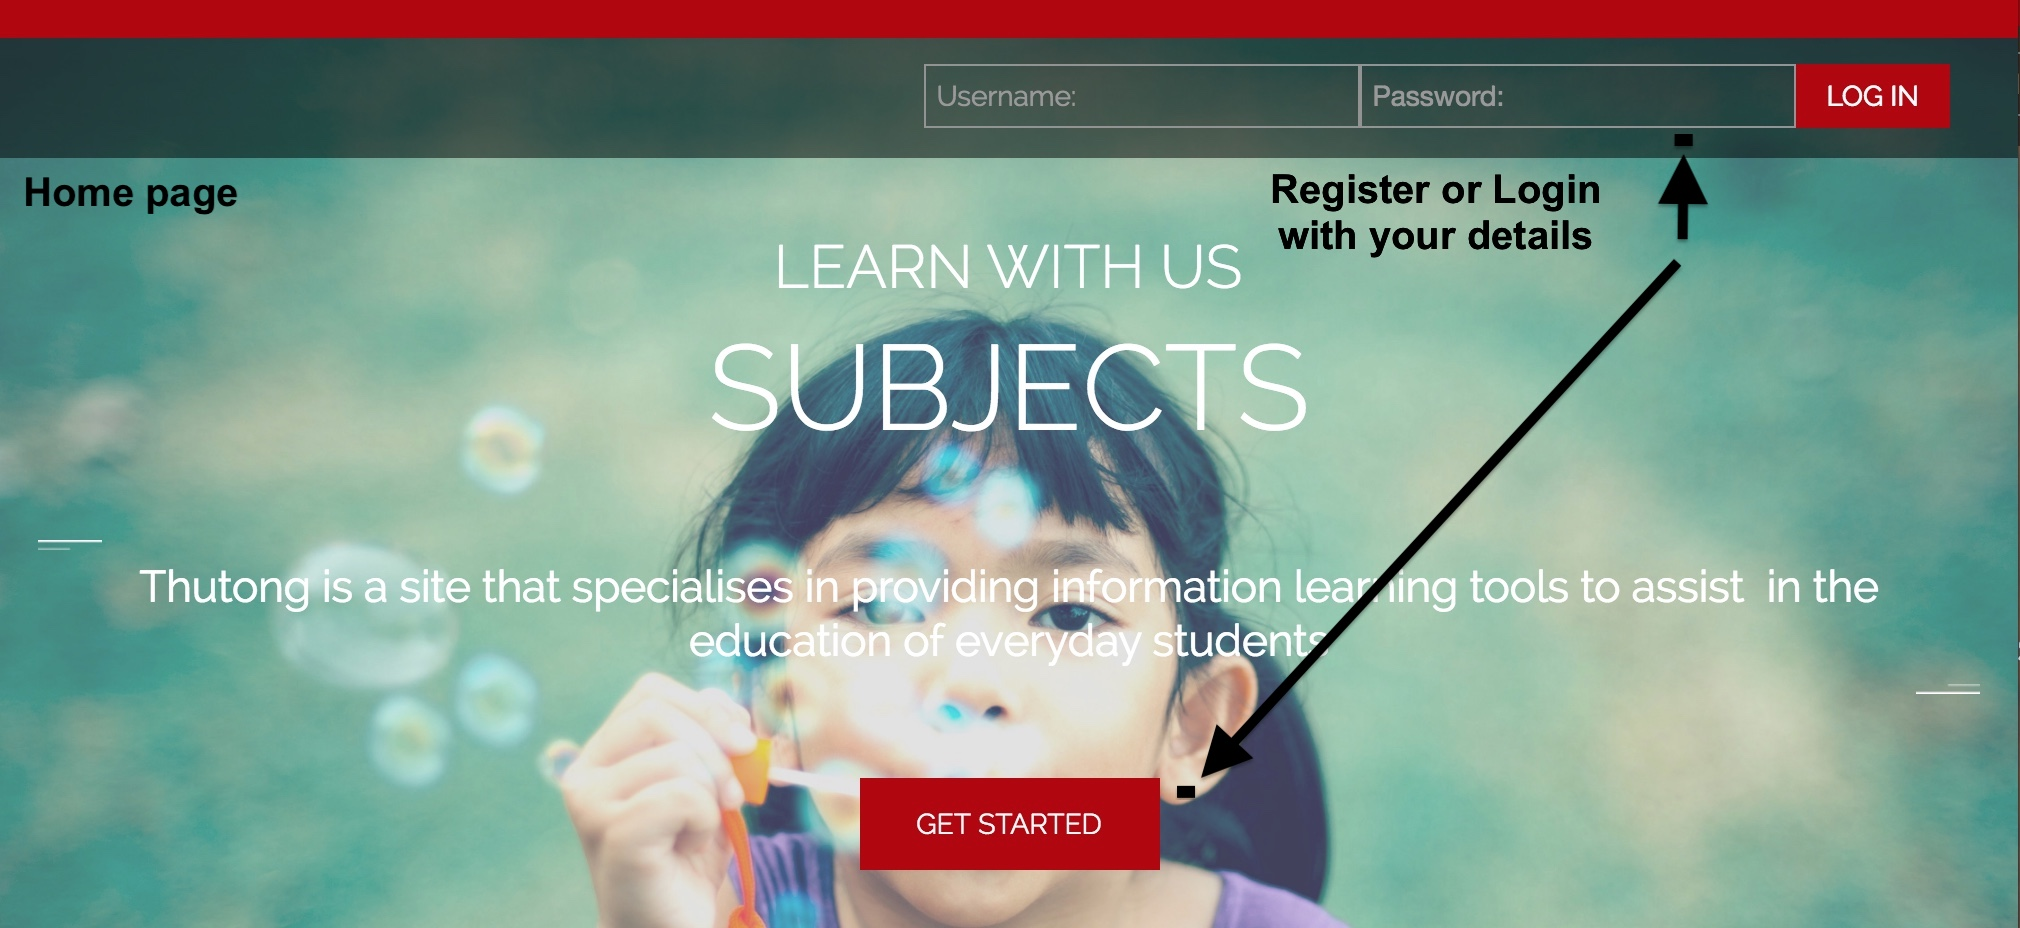
\includegraphics[width=\linewidth]{Pictures/1.jpeg}
Figure 1: Main Thutong page\\\\		
To register or login click go to the main page of the Thutong system.\\\\

\subsubsection{Register}
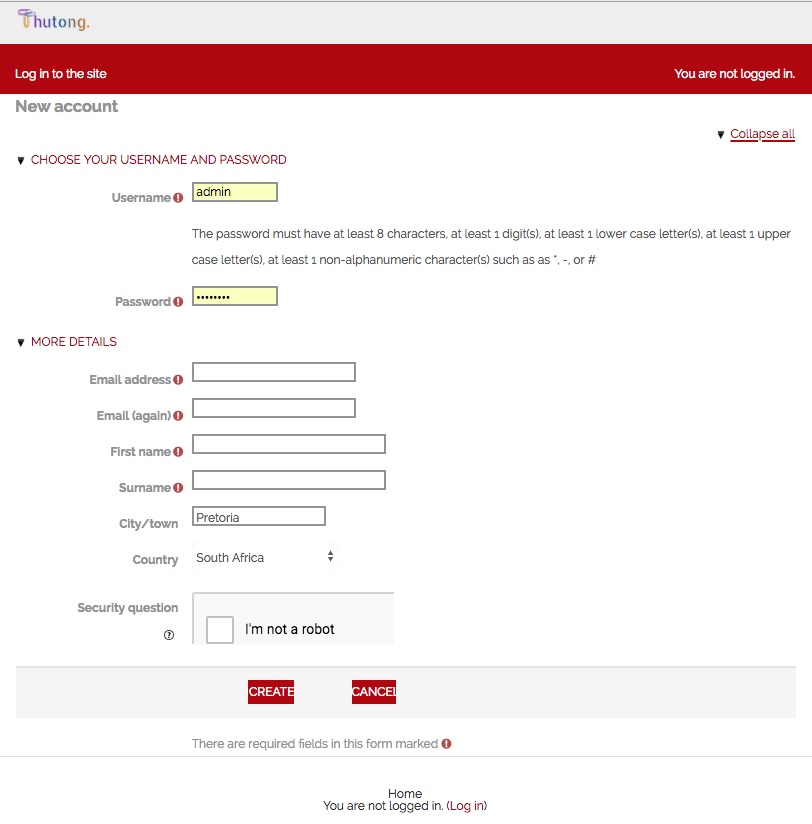
\includegraphics[width=0.8\linewidth]{Pictures/22.jpeg} \\
Figure 1.1: Registration page\\\\
To register click on Get started on the first slide (Subjects) in the carousal as shown in the image above.\\\\

\subsubsection{Login}
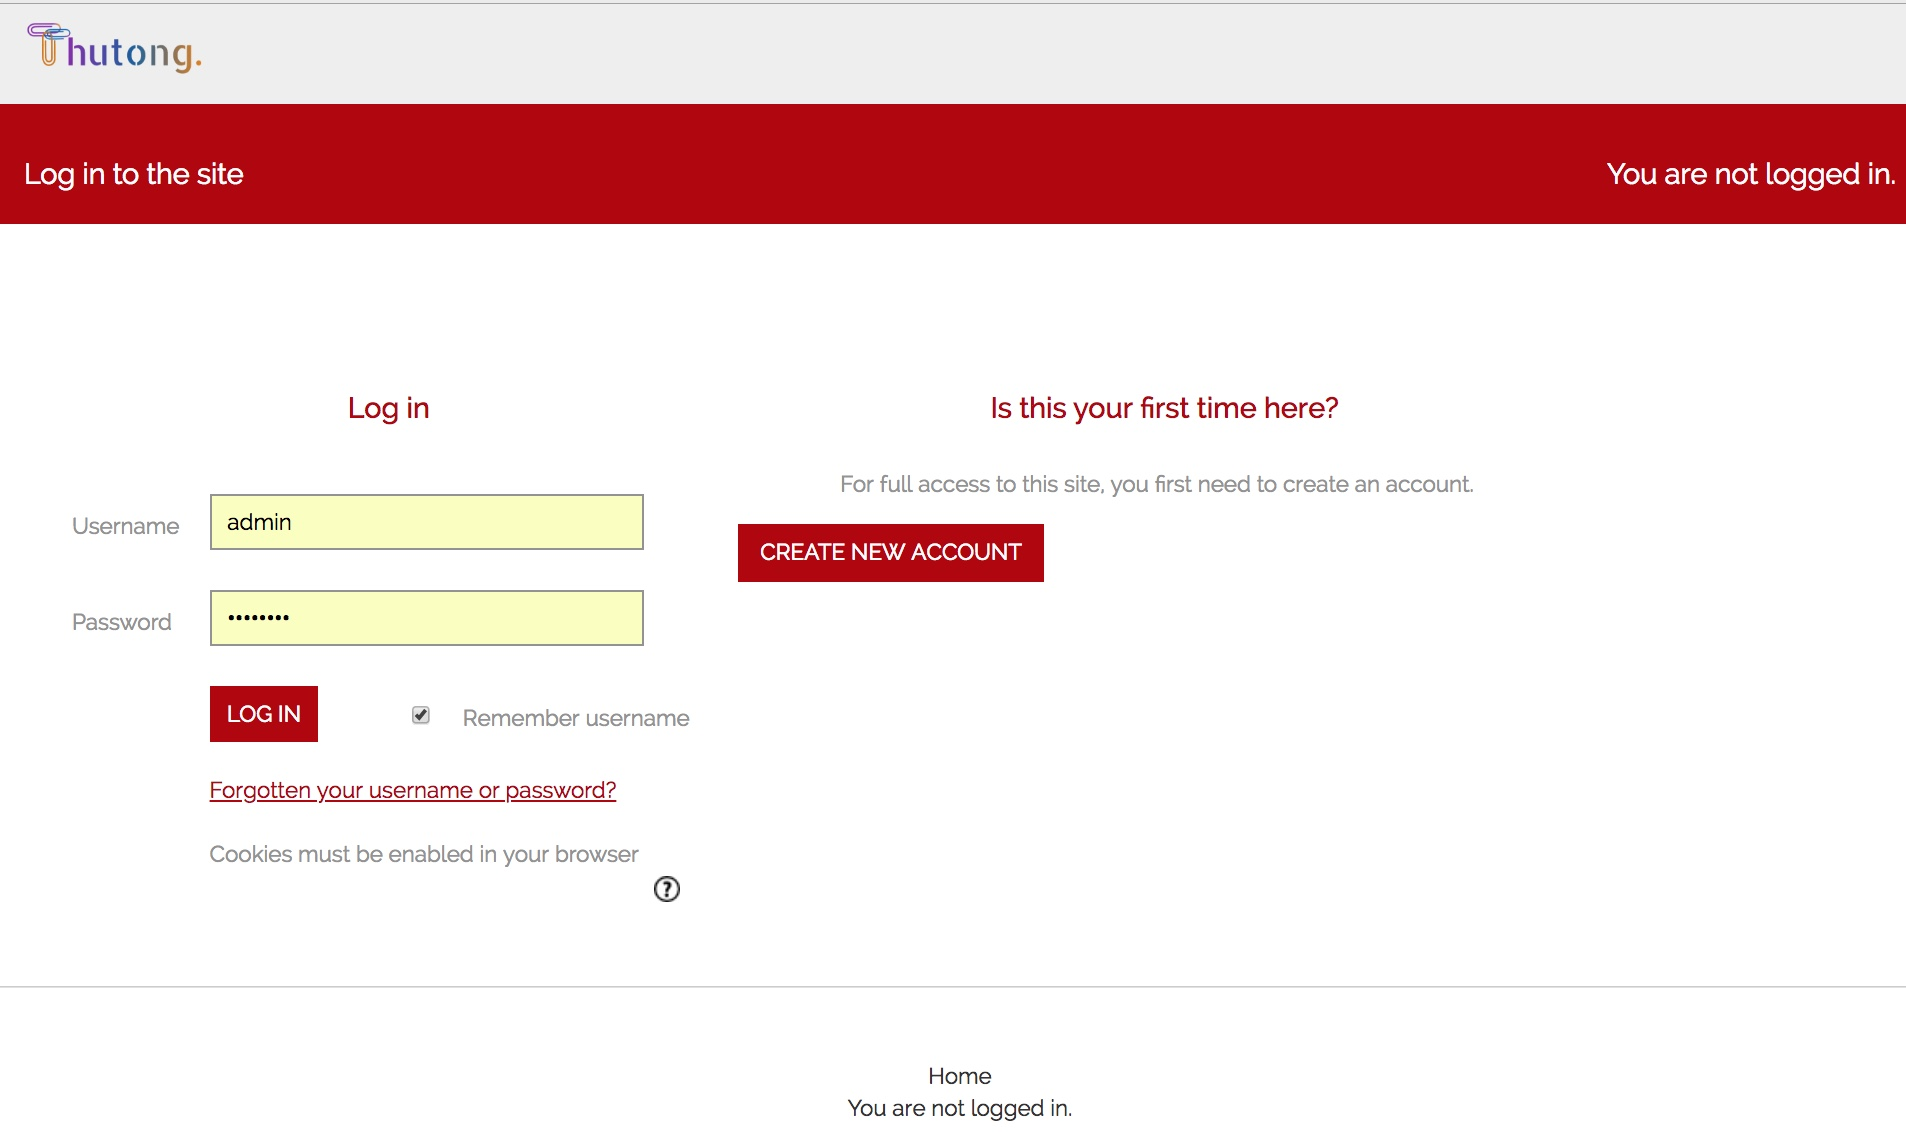
\includegraphics[width=0.8\linewidth]{Pictures/21.jpeg} \\
Figure 1.2: Alternative Login page\\\\
To login, simply login near the site header as show in figure 1 or use the alternative login by clicking "Get started" on the main page.

\subsubsection{Forgotten password}
In the event that a user is unable to login due to a forgotten password or username, the user may click on ”Forgotten your username or password?” such as that shown in figure 1.1 and 1.2. From hereon, the user will be redirected to the page which will alow them to reset their passwords via email. \\\\
They can then search for their accounts based on their username or email address. If either of the 2 result in a successful search, a system generated email will be sent to the email address on record where users will get a pass- word reset link.	

\subsubsection{Login as guest}
To login as guests, visitors must click the ”Login as guest” button on Figure 1.2 above, where they will be redirected to the default guest-login page. Here users will be able to see all courses but may only have access to courses that allow guest access, these are indicated by the circled icon on the bottom right corner of the course.



		\subsection{Access profile}
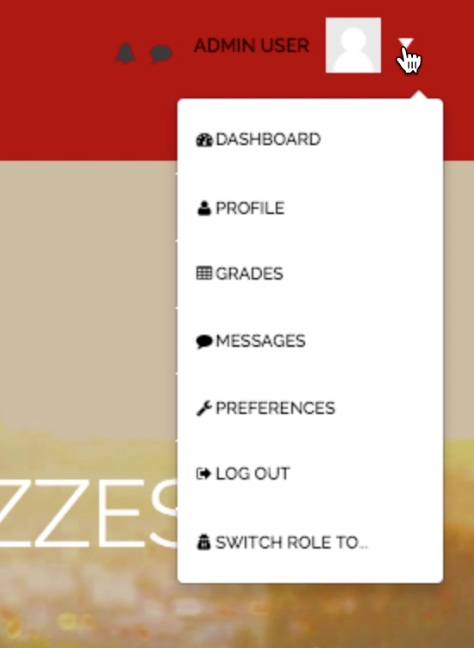
\includegraphics[width=0.2\linewidth]{Pictures/11.jpeg} \\
Figure 2: Access profile drop down \\\\
This manual does not go into the specifics of the moodle courts management system of which it is based.
Therefore this manual will only cover the basic profile element of users. \\\\
In figure 2, to access different aspects of your profile click on the drop down to show your profile option, when the drop down displays like in the image you can view your profile or dashboard or any other necessary profile facets, by just clicking on the relevant links shown.
If you would like to add a profile picture click on the default profile picture in the image.


		\subsection{Dashboard}
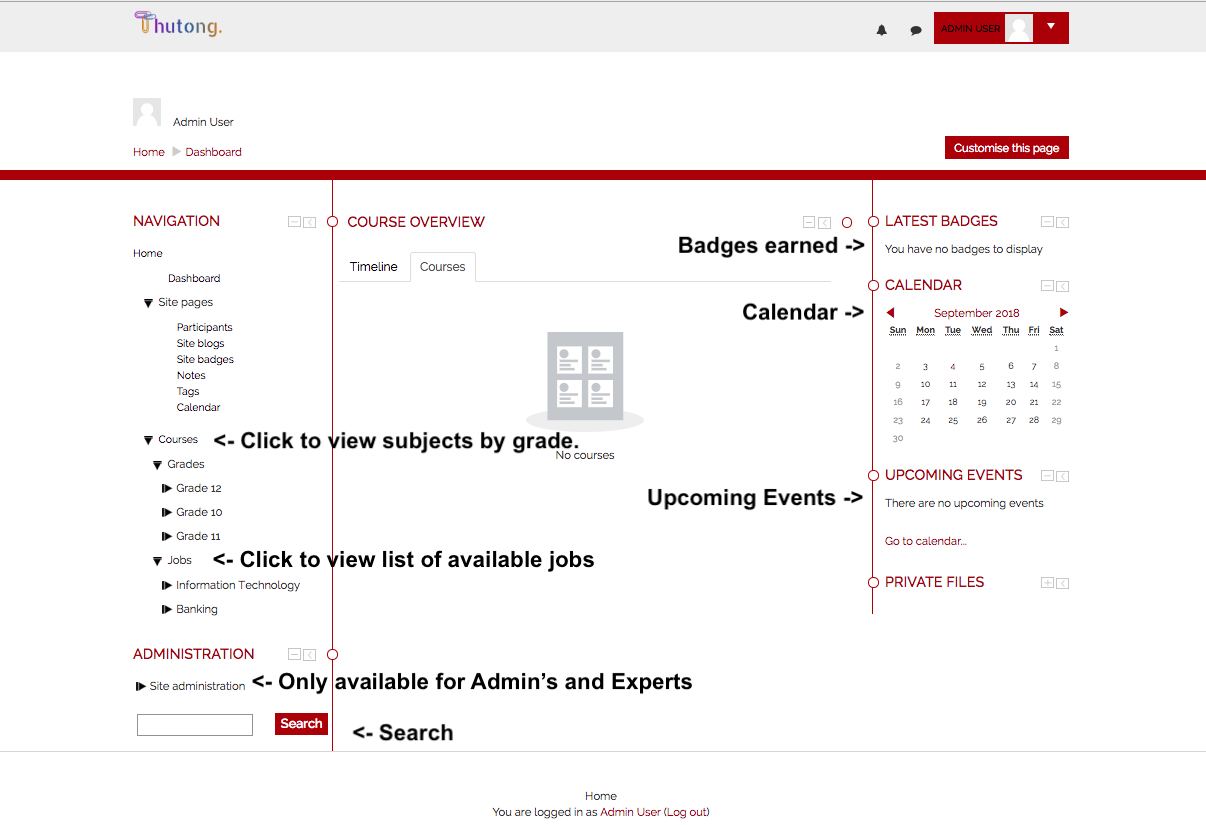
\includegraphics[width=0.6\linewidth]{Pictures/12.png} \\
Figure 3: Basic users dashboard \\\\
Students can see and access subjects by grades, while only Experts and Administration can add content.
Experts however cannot edit main functionality or look of the site, beside adding anything relevant to Thutong or managing content for students to utilize as well as keeping track of certain Student tracking analytic.


\section{Using the system}



		\subsection{Setting up Subjects}
To add subjects or content as an Administrator or educational Expert, you can try one of two options \\
1. Go to Administration \textrightarrow  Click on Course administration \textrightarrow edit setting \textrightarrow add course.\\
2. Click on turn editing on, then select Courses on the left hand side (navigation section), then when it loads, click add course.\\\\
When adding a course ensure to click on the option to add the subject name in the course name textbox, while making sure that it is adding the subject to the correct grade.
Only Administrators and educational experts (teachers) can edit course subjects and content.

		\subsection{Adding Content to Subjects}
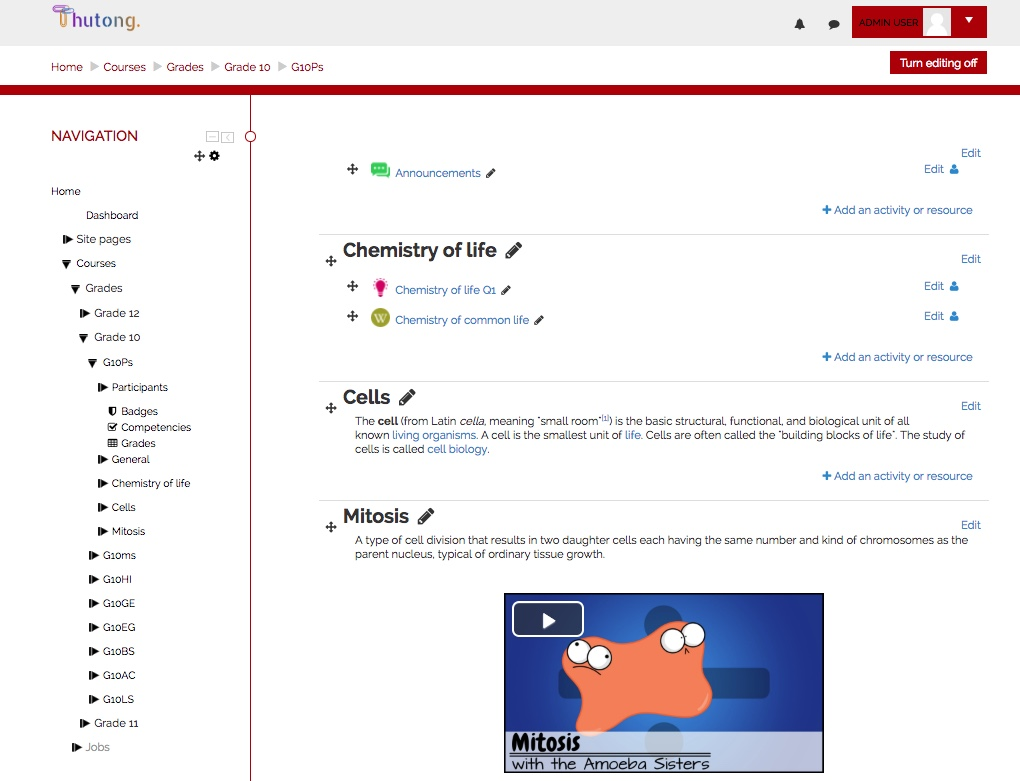
\includegraphics[width=\linewidth]{Pictures/13.jpeg} \\
Figure 4: Basic users dashboard \\\\
In figure 4, you can see an option on the top right hand side that says "Turn editing on", that will allow Administrators or educational experts to add content using a variety of methods such as that shows in the example figure. 

\subsection{Adding Content extended}
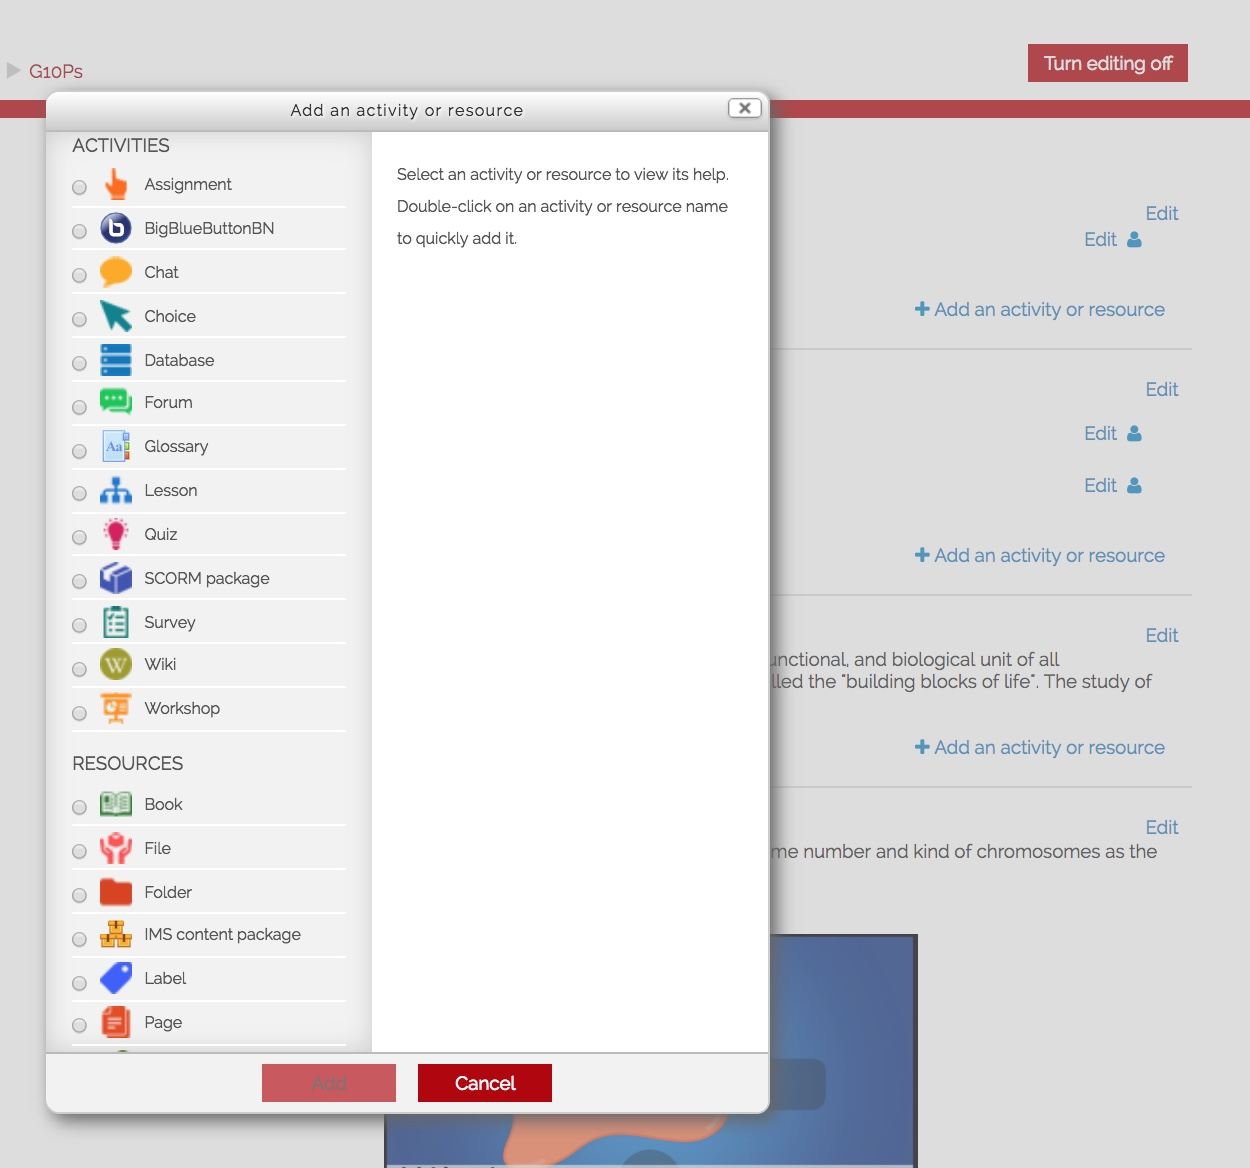
\includegraphics[width=0.6\linewidth]{Pictures/24.jpeg} \\
Figure 4.1: Turn on editing "activity or resources choices selection \\\\
From hereon the Educational Expert (teacher) may click ”add an activity or resource”, or any other possible content that they can add. This is shown in the above. You can then click ”lesson” to add a lesson or other ”interactive content” to add a more interactive lesson or learning tools such as a quiz. \\\\
After adding an activity or resource, you will be shown all other possible options from how long the lesson should last to who it should be available to with the ability to manage or edit these activities or lessons within a course. Once finished with completing a subject with all of its data , one can then save and return to the subjects main page or view the lesson that was just added which is shown in figure 4. \\\\

\subsubsection{Specific activities example}
Example
In order to add assessment activity, a teacher would follow exactly the same steps as adding a lesson above, however instead of clicking ”lesson” on Figure 4, they can then just click the specific activity they wish to add, for instance ”quiz”, and also proceed in a similar manner as Figure 4.1 above.

\subsubsection{Completing a quiz}
A very similar task to the one viewing a lesson above. Follow the exact same instructions as in section 5.2.1 above. The only difference in this case is you will be exposed to the quiz page, where you can partake in the quiz as shown in Figure 11 below.

\subsubsection{Using the topic discussion board}
The course discussion board, if made available by the teacher will appear in the same manner as the quiz and lesson above. The steps to accessing it are very similar to both activities completed above.

	
\subsection{Backing up or transferring Course content}

\subsubsection{To backup a course}

Go into the course. \\\\
1. Click the Backup link either in the gear menu or the Administration block.\\
2. Initial settings - Select activities, blocks, filters and other items as required then click the Next button. \\ 
3. Users with appropriate permissions, such as administrators and managers, can choose whether to include users, anonymity user information, or include user role assignments, groups, groupings, user files, comments, user completion details, course logs and grade history in the backup.\\
4. Schema settings - Select/deselect specific items to include in backup, then click the Next button.\\
5. If desired, select specific types of activity to be backed up by clicking the link 'Show type options'\\
6. Confirmation and review - Check that everything is as required, using the Previous button if necessary, otherwise click the 'Perform backup' button.\\
7. Complete - Click the Continue button

\subsubsection{Restoring a course}
To restore courses go to Administration > Course administration > Restore and select the Thutong moodle course files to restore.





		\section{Additions to the Thutong system}
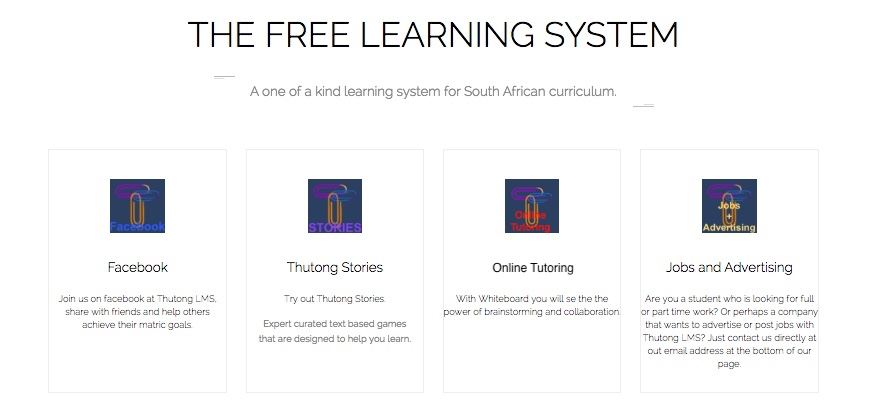
\includegraphics[width=\linewidth]{Pictures/2.jpeg} \\
Figure 5: Additions to moodle \\\\
\subsection{Facebook}

As any user, to access the Thutong LMS facebook page just click on any Facebook icon or card as shown above. \\
Students may ask questions on the Thutong Facebook pages and get any updated and relevant Thutong LMS information.
The Facebook page has been set up to include chat-bot integration that can answer simple questions about Thutong when an educational Expert is not available to assist them.

\subsection{Thutong Stories}

Thutong stories is a simple subsystem that allows users to play simple text based multiple choice based games, that can be made to keep track of a users statistics as they play through the game of their choice as well as restart button to reset the game back to the main choice screen to enable a user to choose a game to play. \\
Each game is based on different subjects such as Maths or science, with the game getting harder and more complex over time, and the actions of the user affecting the outcome of the game. The name of the game loosely indicates the subject on which the game of choice will be based on. \\
Thutong stories also has settings to allow students who play its games to edit the way they seen the text based content when clicking on the settings button. \\\\ Thutong Stories is unique when it comes to its ability to promote text based learning by allowing students to learn by playing a game that can test their knowledge on a specific subject. 
\\\\
ChoiceScript LLC created a simple scripting language that runs on any mobile or web platform called ChoiceScript games which provides the ability for Thutong to provide fun text based games to users for non commercial purposes.
\\\\
If a student wishes to add to Thutong Stories list of games they can go to www.choicescriptdev.wikia.com and learn how to script a game and email it to Thutong general email account for consideration. (i.e. Thutong email account is listed at the bottom of the main website systems page.)


\subsection{Whiteboard or Thutong Uber Tutors}

TO BE COMPLETED\\\\
TO BE COMPLETED\\\\\
TO BE COMPLETED\\\\\
TO BE COMPLETED\\\\\
TO BE COMPLETED\\\\\
TO BE COMPLETED\\\\\
TO BE COMPLETED\\\\\
TO BE COMPLETED\\\\\
TO BE COMPLETED\\\\

\subsection{Jobs/Subjects and Sponsored Advertising}

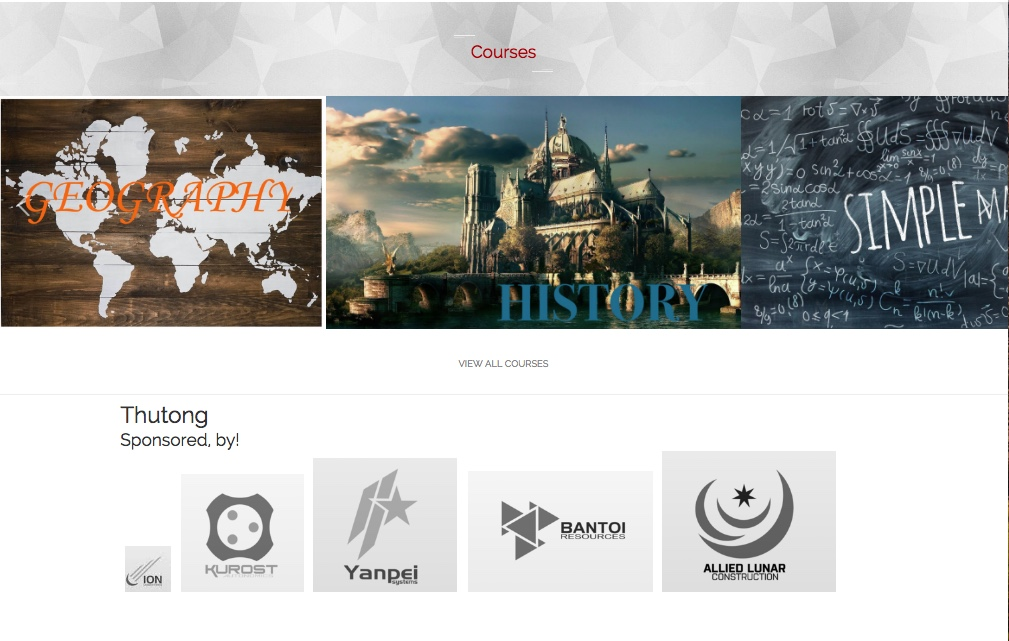
\includegraphics[width=\linewidth]{Pictures/3.jpeg} \\
Figure 6: Sponsored Advertising \\\\
Companies can email Thutong with regard to Advertising their business on Thutong LMS main page as seen in figure 7 above.\\\\
Administrators can add the logos or messages provided by these companies into the Sponsored by section of Thutong by going to the main page and clicking the "Turn on editing" setting button and clicking on the gear icon that pops up for that section to open up the edit screen. When editing the section you can add a picture simply by clicking "add image" and following the steps. \\\\
Administrators and Educational experts can also adjust the Course carousal above the Sponsored section to show different subject images.


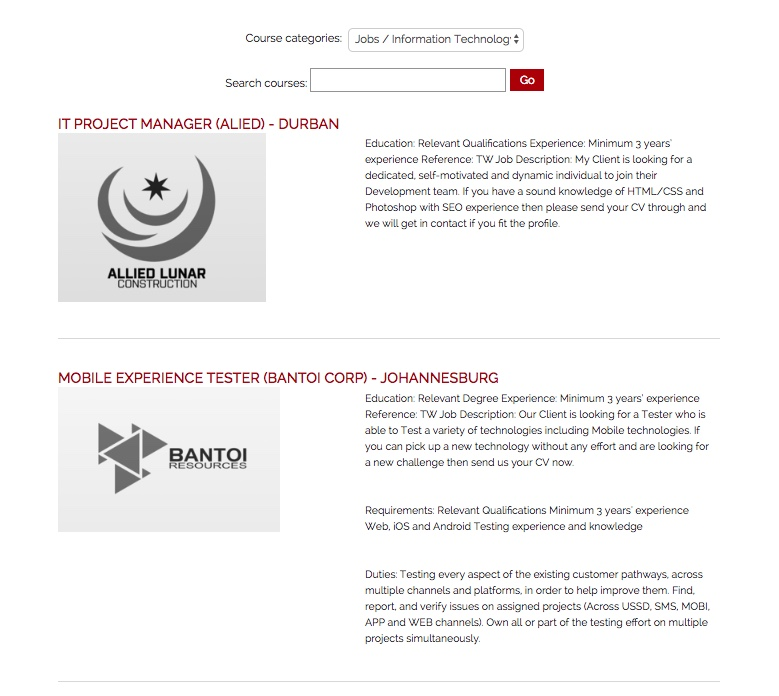
\includegraphics[width=\linewidth]{Pictures/14.jpeg} \\
Figure 7: Jobs list \\\\
Administrators can add jobs to the Thutong Jobs list. This can be done by adding a job in the same way one can add a subject to a grade like that which is described in the "Adding Content to Subjects", except Jobs will be added to the Jobs list instead as if it where a course.\\\\
Student who are looking for full or part time work can go to and see a set of available jobs list (such as that in figure 7) of available jobs by going to their course page -> courses -> and clicking on Jobs; this can also be accessed near the bottom of the main Thutong page.  \\\\ Should a  company that wants to advertise or post jobs with Thutong LMS? Just contact us directly at out email address at the bottom of our page.

		
	
\section{Basic Troubleshooting}
If you're using Chrome or Firefox to view a page with mixed content (HTTPS and HTTP), the page or content may be blocked by a browser security feature. \\ Disable this feature or use a different browser.\\\\
An Error Has Occurred; internal server error. Or any other errors can be resolved just contact the Admin or Education expert at ThutongLearning11@gmail.com. \\\\
Administrator can reference the large online support community with regard to any Moodle side Thutong errors.

TO BE COMPLETED\\\\TO BE COMPLETED\\\\TO BE COMPLETED\\\\TO BE COMPLETED\\\\TO BE COMPLETED\\\\TO BE COMPLETED\\\\TO BE COMPLETED\\\\TO BE COMPLETED\\\\
\end{document}
